\documentclass{beamer}
\usepackage{amsmath, amssymb}
\usepackage{graphicx}
\usepackage[inline]{asymptote}
\usepackage{hyperref}

\title{Luck: A more natural statistic}
\author{Warren D. MacEvoy}
\date{\today}

\begin{document}

\frame{\titlepage}

% Slide 1: Introduction
\begin{frame}
\frametitle{Introduction to Luck}
\begin{itemize}
    \item \textbf{What is Luck?}
        \begin{itemize}
            \item Luck quantifies how likely an outcome is compared to others.
            \item Formal definition:
              \[|\Omega(x)| = \text{Prob}(\text{outcomes more likely than $x$})\]
              \[|\omega(x)| = \text{Prob}(\text{outcomes equally likely to $x$})\]
            \[L(x) = |\Omega(x)| + \frac{1}{2}|\omega(x)|\]
        \end{itemize}
    \item \textbf{Range of Luck:} 0 (unlucky) to 1 (very lucky), average luck is 0.5.
    \item \textbf{Why Study Luck?}
        \begin{itemize}
            \item Luck connects mathematical probability to real-world scenarios.
            \item Examples: Password guessing, dating, randomness.
        \end{itemize}
\end{itemize}
\end{frame}

% Slide 2: Example: Luck in Coin Tosses
\begin{frame}
\frametitle{Example: Luck in Coin Tosses}
\begin{itemize}
    \item Consider 8 fair coin flips.
    \item What is the luck of getting exactly 4 heads?
    \[
    p(x) = \frac{8!}{x!(8-x)!} \left( \frac{1}{2} \right)^8
    \]
    \item Luck for different outcomes is computed using the binomial distribution.
    \item \textbf{Table:} Luck values for outcomes
    \begin{center}
    \begin{tabular}{|c|c|c|c|c|c|c|c|}
    \hline
    $x$ & $p(x)$ & $\Omega(x)$ & $|\Omega(x)|$ & $\omega(x)$ & $|\omega(x)|$ & $L(x)$ \\
    \hline
     4 & 0.2734 &  \{\} & 0.0000 & \{4\} & 0.2734 & 0.1367 \\
3 or 5 & 0.2188 & \{4\} & 0.2734 & \{3,5\} & 0.4375 & 0.4922 \\
2 or 6 & 0.1094 & \{3,\ldots,5\} & 0.7109 & \{2,6\} & 0.2188 & 0.8203 \\
1 or 7 & 0.0313 & \{2,\ldots,6\} & 0.9297 & \{1,7\} & 0.0625 & 0.9609 \\
0 or 8 & 0.0039 & \{1,\ldots,7\} & 0.9922 & \{0,8\} & 0.0078 & 0.9961 \\
    \hline
    \end{tabular}
    \end{center}
\end{itemize}
\end{frame}

% Slide 3: Normal Distribution and Luck
\begin{frame}
  \frametitle{Luck in the Normal Distribution}
  In large dimensions, normal observations are {\em not} crowded near $x \approx \mu$, but almost certainly ($99.99\%$) within $\pm 3$ of the elliptical shell
  \[
    |\Sigma^{-1/2}(x-\mu)|=\sqrt{d_f-1/2} \,.
  \]
This is a pretty good statement even for $d_f$ of 3....
\end{frame}

\begin{frame}
\frametitle{$N=1$ statistics}
\begin{center}
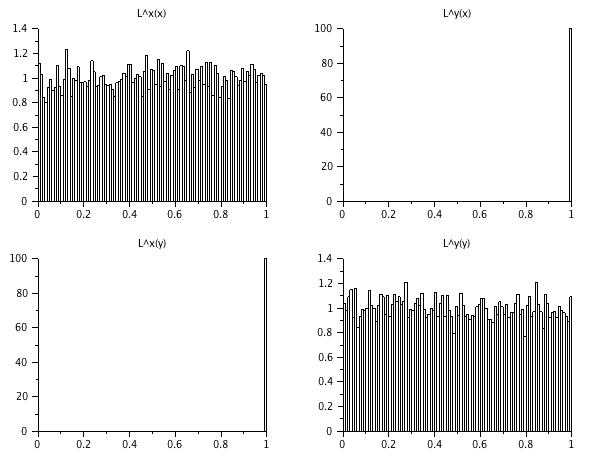
\includegraphics[width=0.75\textwidth]{img/normal}
\end{center}
\end{frame}

% Slide 6: Z-Luck and its Applications
\begin{frame}
\frametitle{Z-Luck: Combining Luck from Experiments}
\begin{itemize}
    \item Z-luck allows us to combine results from multiple independent experiments.
    \item Formula for z-luck:
    \[
    z_L = \sqrt{\|\Sigma^{-1}(x - \mu)\|} - \sqrt{d_f - \frac{1}{2}}
    \]
    \item Example: Combining observations from normal distributions across different dimensions.
    \item Application in determining whether results from independent experiments align or not.
\end{itemize}
\end{frame}

\begin{frame}
  \frametitle{Coin Luck: Natural Unit for Luck}
  \[ L_C(x) = \log_2 \frac{L(x)}{1-L(x)} \]

  This is expressing luck in ``coin tosses'' where negative is bad luck (nearly zero) and positive is good luck (nearly one).
\end{frame}

% Slide 8: Conclusion
\begin{frame}
\frametitle{Conclusion}
\begin{itemize}
    \item Luck is a versatile concept connecting probability and real-world events.
    \item Applications range from testing randomness to real-world problem-solving.
    \item Key insights:
        \begin{itemize}
            \item Uniformity of luck across distributions.
            \item Elliptical shell behavior in multinomial distributions.
        \end{itemize}
    \item Thank you! Questions?
\end{itemize}
\end{frame}

\end{document}
